%% Auto-generated by fig_qualitative.py -- do not edit by hand.
\documentclass[border=0pt]{standalone}
\usepackage{iftex}
\ifPDFTeX
  \usepackage[T1]{fontenc}\usepackage{times}
\else
  \usepackage{fontspec}\setmainfont{texgyretermes}[Extension=.otf,UprightFont=*-regular,BoldFont=*-bold,ItalicFont=*-italic,BoldItalicFont=*-bolditalic]
\fi
\usepackage{graphicx}
\usepackage{tikz}
% Shared method colors for all figures/diagrams (same hexes as figures/src/figstyle.py).
% Validated colorblind-safe on white (all-pairs CVD dE >= 9.4, contrast >= 3.4:1); always pair with a
% second cue (marker shape, label) so identity never relies on hue alone.
\definecolor{cOurs}{HTML}{256ABF}      % KalSea (gate + Kalman forecaster + predictor-corrector gap smoothing)
\definecolor{cKalSea}{HTML}{199E70}    % KalSea (Kalman forecasting, no smoothing)
\definecolor{cSeaCache}{HTML}{D95926}  % SeaCache (SEA gate + residual reuse)
\definecolor{cReference}{HTML}{0B0B0B} % 50-step reference
\definecolor{cInk}{HTML}{0B0B0B}
\definecolor{cInkTwo}{HTML}{52514E}
\definecolor{cMuted}{HTML}{898781}
\definecolor{cGrid}{HTML}{E1E0D9}

\newcommand{\hdr}{\fontsize{7.5}{8.5}\selectfont}
\newcommand{\sub}{\fontsize{7}{8}\selectfont\color{cInkTwo}}
\newcommand{\prm}{\fontsize{7}{8.1}\selectfont\itshape\color{cInk}}
\newcommand{\num}{\fontsize{7}{8}\selectfont\color{cInk}}
\begin{document}
\begin{tikzpicture}[x=1bp,y=1bp,line join=round]
\path[use as bounding box] (0,0) rectangle (495.00,-322.50);
\node[anchor=south,inner sep=0] at (49.25,-21.80) {\hdr Reference};
\node[anchor=south,inner sep=0] at (49.25,-11.40) {\sub 50 NFE};
\draw[cMuted,line width=0.4bp] (11.00,-12.40) -- (87.50,-12.40);
\node[anchor=south,inner sep=0] at (169.25,-11.40) {\sub 13 NFE, identical computed steps};
\draw[cMuted,line width=0.4bp] (91.00,-12.40) -- (247.50,-12.40);
\node[anchor=south,inner sep=0] (h01) at (132.25,-21.80) {\hdr SeaCache};
\path (h01.west) ++(-4.0,1.9) coordinate (mk);
\begin{scope}[shift={(mk)}]\fill[cSeaCache] (-2.10,-2.10) rectangle (2.10,2.10);\end{scope}
\node[anchor=south,inner sep=0] (h02) at (212.25,-21.80) {\hdr KalSea};
\path (h02.west) ++(-4.0,1.9) coordinate (mk);
\begin{scope}[shift={(mk)}]\fill[cOurs] (0.00,-0.25) circle (2.21);\end{scope}
\node[anchor=south,inner sep=0] at (295.75,-21.80) {\hdr Reference};
\node[anchor=south,inner sep=0] at (295.75,-11.40) {\sub 50 NFE};
\draw[cMuted,line width=0.4bp] (257.50,-12.40) -- (334.00,-12.40);
\node[anchor=south,inner sep=0] at (415.75,-11.40) {\sub 13 NFE, identical computed steps};
\draw[cMuted,line width=0.4bp] (337.50,-12.40) -- (494.00,-12.40);
\node[anchor=south,inner sep=0] (h11) at (378.75,-21.80) {\hdr SeaCache};
\path (h11.west) ++(-4.0,1.9) coordinate (mk);
\begin{scope}[shift={(mk)}]\fill[cSeaCache] (-2.10,-2.10) rectangle (2.10,2.10);\end{scope}
\node[anchor=south,inner sep=0] (h12) at (458.75,-21.80) {\hdr KalSea};
\path (h12.west) ++(-4.0,1.9) coordinate (mk);
\begin{scope}[shift={(mk)}]\fill[cOurs] (0.00,-0.25) circle (2.21);\end{scope}
\node[anchor=south west,inner sep=0,text width=238.50bp,align=flush left,font=\prm] at (10.00,-40.50) {``A couch on the left of a chair.''};
\node[anchor=north west,inner sep=0] at (10.00,-42.50) {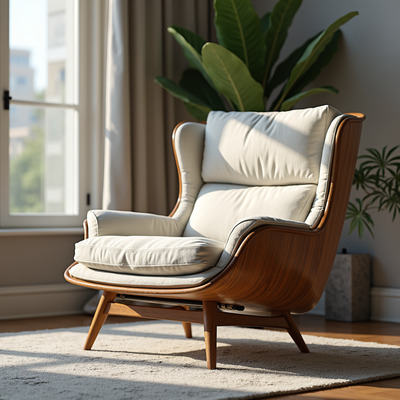
\includegraphics[width=78.500bp,height=78.500bp]{qual_tiles/nfe13/125_reference_full.jpg}};
\draw[black,line width=1.3bp] (28.40,-94.63) rectangle (48.02,-104.44);
\draw[white,line width=0.6bp] (28.40,-94.63) rectangle (48.02,-104.44);
\node[anchor=north west,inner sep=0] at (10.00,-122.50) {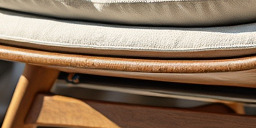
\includegraphics[width=78.500bp,height=39.250bp]{qual_tiles/nfe13/125_reference_crop.jpg}};
\node[anchor=north,inner sep=0] at (49.25,-163.55) {\num\color{cInkTwo}PSNR (dB)};
\node[anchor=north west,inner sep=0] at (90.00,-42.50) {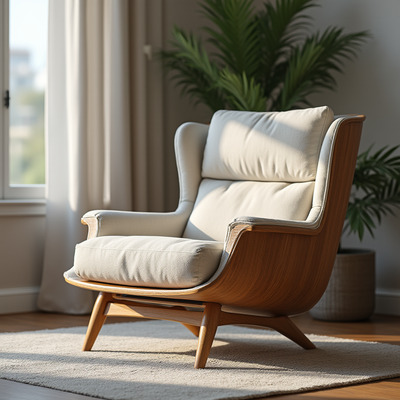
\includegraphics[width=78.500bp,height=78.500bp]{qual_tiles/nfe13/125_seacache_full.jpg}};
\draw[black,line width=1.3bp] (108.40,-94.63) rectangle (128.02,-104.44);
\draw[white,line width=0.6bp] (108.40,-94.63) rectangle (128.02,-104.44);
\node[anchor=north west,inner sep=0] at (90.00,-122.50) {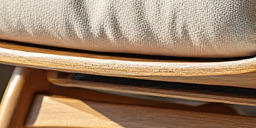
\includegraphics[width=78.500bp,height=39.250bp]{qual_tiles/nfe13/125_seacache_crop.jpg}};
\node[anchor=north,inner sep=0] at (129.25,-163.55) {\num 19.09};
\node[anchor=north west,inner sep=0] at (170.00,-42.50) {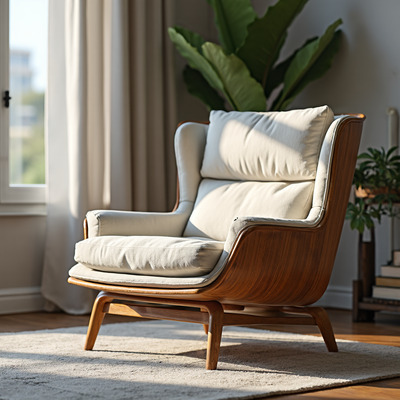
\includegraphics[width=78.500bp,height=78.500bp]{qual_tiles/nfe13/125_ours_full.jpg}};
\draw[black,line width=1.3bp] (188.40,-94.63) rectangle (208.02,-104.44);
\draw[white,line width=0.6bp] (188.40,-94.63) rectangle (208.02,-104.44);
\node[anchor=north west,inner sep=0] at (170.00,-122.50) {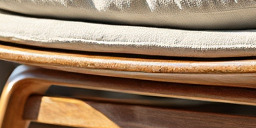
\includegraphics[width=78.500bp,height=39.250bp]{qual_tiles/nfe13/125_ours_crop.jpg}};
\node[anchor=north,inner sep=0] at (209.25,-163.55) {\num \textbf{20.27}};
\node[rotate=90,anchor=south,inner sep=0] at (6.80,-102.12) {\sub Median gain};
\node[anchor=south west,inner sep=0,text width=238.50bp,align=flush left,font=\prm] at (256.50,-40.50) {``McDonalds Church.''};
\node[anchor=north west,inner sep=0] at (256.50,-42.50) {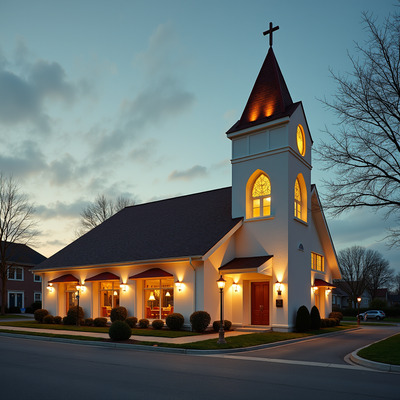
\includegraphics[width=78.500bp,height=78.500bp]{qual_tiles/nfe13/154_reference_full.jpg}};
\draw[black,line width=1.3bp] (273.06,-92.79) rectangle (292.68,-102.60);
\draw[white,line width=0.6bp] (273.06,-92.79) rectangle (292.68,-102.60);
\node[anchor=north west,inner sep=0] at (256.50,-122.50) {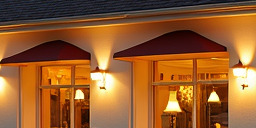
\includegraphics[width=78.500bp,height=39.250bp]{qual_tiles/nfe13/154_reference_crop.jpg}};
\node[anchor=north,inner sep=0] at (295.75,-163.55) {\num\color{cInkTwo}PSNR (dB)};
\node[anchor=north west,inner sep=0] at (336.50,-42.50) {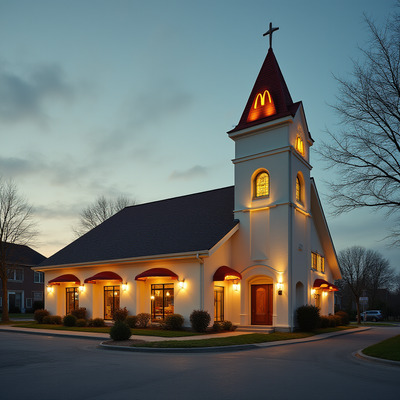
\includegraphics[width=78.500bp,height=78.500bp]{qual_tiles/nfe13/154_seacache_full.jpg}};
\draw[black,line width=1.3bp] (353.06,-92.79) rectangle (372.68,-102.60);
\draw[white,line width=0.6bp] (353.06,-92.79) rectangle (372.68,-102.60);
\node[anchor=north west,inner sep=0] at (336.50,-122.50) {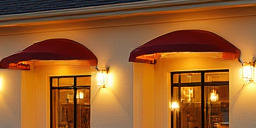
\includegraphics[width=78.500bp,height=39.250bp]{qual_tiles/nfe13/154_seacache_crop.jpg}};
\node[anchor=north,inner sep=0] at (375.75,-163.55) {\num 21.49};
\node[anchor=north west,inner sep=0] at (416.50,-42.50) {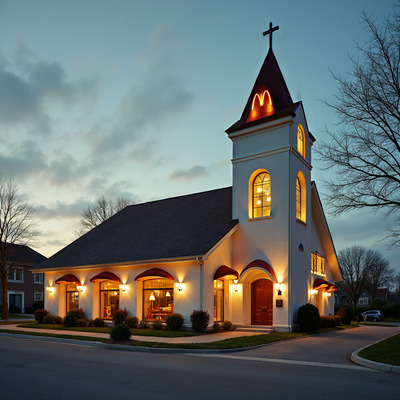
\includegraphics[width=78.500bp,height=78.500bp]{qual_tiles/nfe13/154_ours_full.jpg}};
\draw[black,line width=1.3bp] (433.06,-92.79) rectangle (452.68,-102.60);
\draw[white,line width=0.6bp] (433.06,-92.79) rectangle (452.68,-102.60);
\node[anchor=north west,inner sep=0] at (416.50,-122.50) {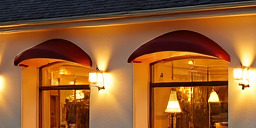
\includegraphics[width=78.500bp,height=39.250bp]{qual_tiles/nfe13/154_ours_crop.jpg}};
\node[anchor=north,inner sep=0] at (455.75,-163.55) {\num \textbf{22.69}};
\node[anchor=south west,inner sep=0,text width=238.50bp,align=flush left,font=\prm] at (10.00,-192.75) {``Four cars on the street.''};
\node[anchor=north west,inner sep=0] at (10.00,-194.75) {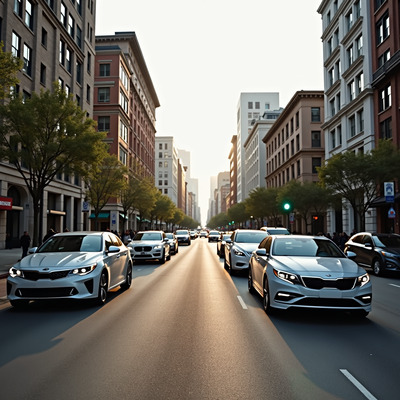
\includegraphics[width=78.500bp,height=78.500bp]{qual_tiles/nfe13/038_reference_full.jpg}};
\draw[black,line width=1.3bp] (67.65,-205.18) rectangle (87.27,-214.99);
\draw[white,line width=0.6bp] (67.65,-205.18) rectangle (87.27,-214.99);
\node[anchor=north west,inner sep=0] at (10.00,-274.75) {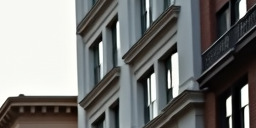
\includegraphics[width=78.500bp,height=39.250bp]{qual_tiles/nfe13/038_reference_crop.jpg}};
\node[anchor=north,inner sep=0] at (49.25,-315.80) {\num\color{cInkTwo}PSNR (dB)};
\node[anchor=north west,inner sep=0] at (90.00,-194.75) {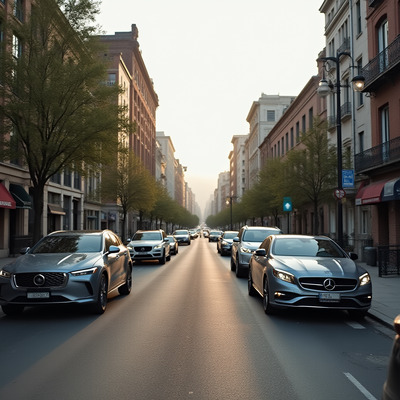
\includegraphics[width=78.500bp,height=78.500bp]{qual_tiles/nfe13/038_seacache_full.jpg}};
\draw[black,line width=1.3bp] (147.65,-205.18) rectangle (167.27,-214.99);
\draw[white,line width=0.6bp] (147.65,-205.18) rectangle (167.27,-214.99);
\node[anchor=north west,inner sep=0] at (90.00,-274.75) {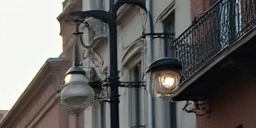
\includegraphics[width=78.500bp,height=39.250bp]{qual_tiles/nfe13/038_seacache_crop.jpg}};
\node[anchor=north,inner sep=0] at (129.25,-315.80) {\num 16.77};
\node[anchor=north west,inner sep=0] at (170.00,-194.75) {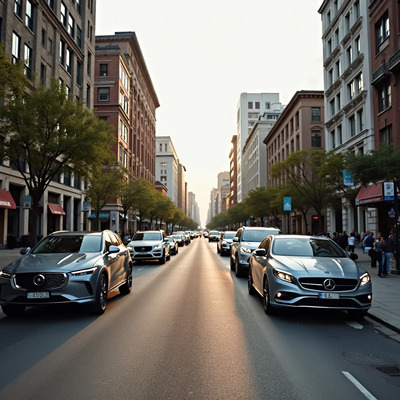
\includegraphics[width=78.500bp,height=78.500bp]{qual_tiles/nfe13/038_ours_full.jpg}};
\draw[black,line width=1.3bp] (227.65,-205.18) rectangle (247.27,-214.99);
\draw[white,line width=0.6bp] (227.65,-205.18) rectangle (247.27,-214.99);
\node[anchor=north west,inner sep=0] at (170.00,-274.75) {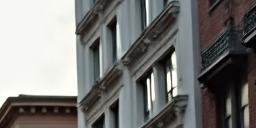
\includegraphics[width=78.500bp,height=39.250bp]{qual_tiles/nfe13/038_ours_crop.jpg}};
\node[anchor=north,inner sep=0] at (209.25,-315.80) {\num \textbf{19.16}};
\node[rotate=90,anchor=south,inner sep=0] at (6.80,-254.38) {\sub Upper-quartile gain};
\node[anchor=south west,inner sep=0,text width=238.50bp,align=flush left,font=\prm] at (256.50,-192.75) {``A triangular orange picture frame. An orange picture frame in the shape of a triangle.''};
\node[anchor=north west,inner sep=0] at (256.50,-194.75) {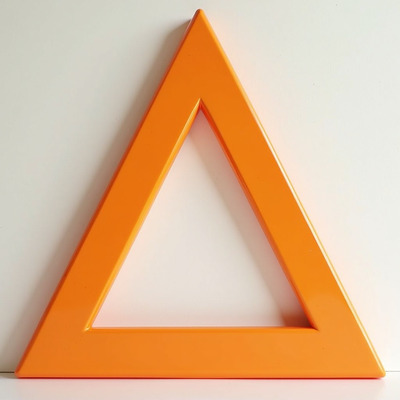
\includegraphics[width=78.500bp,height=78.500bp]{qual_tiles/nfe13/055_reference_full.jpg}};
\draw[black,line width=1.3bp] (289.62,-259.76) rectangle (309.24,-269.57);
\draw[white,line width=0.6bp] (289.62,-259.76) rectangle (309.24,-269.57);
\node[anchor=north west,inner sep=0] at (256.50,-274.75) {
\includegraphics[width=78.500bp,height=39.250bp]{qual_tiles/nfe13/055_reference_crop.jpg}};
\node[anchor=north,inner sep=0] at (295.75,-315.80) {\num\color{cInkTwo}PSNR (dB)};
\node[anchor=north west,inner sep=0] at (336.50,-194.75) {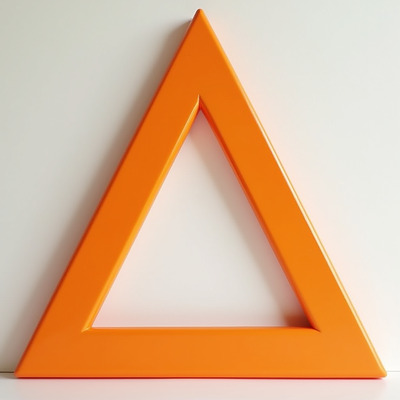
\includegraphics[width=78.500bp,height=78.500bp]{qual_tiles/nfe13/055_seacache_full.jpg}};
\draw[black,line width=1.3bp] (369.62,-259.76) rectangle (389.24,-269.57);
\draw[white,line width=0.6bp] (369.62,-259.76) rectangle (389.24,-269.57);
\node[anchor=north west,inner sep=0] at (336.50,-274.75) {
\includegraphics[width=78.500bp,height=39.250bp]{qual_tiles/nfe13/055_seacache_crop.jpg}};
\node[anchor=north,inner sep=0] at (375.75,-315.80) {\num 33.79};
\node[anchor=north west,inner sep=0] at (416.50,-194.75) {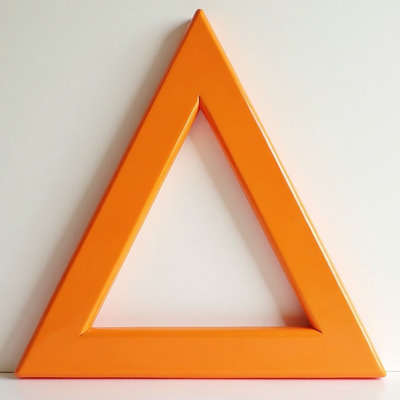
\includegraphics[width=78.500bp,height=78.500bp]{qual_tiles/nfe13/055_ours_full.jpg}};
\draw[black,line width=1.3bp] (449.62,-259.76) rectangle (469.24,-269.57);
\draw[white,line width=0.6bp] (449.62,-259.76) rectangle (469.24,-269.57);
\node[anchor=north west,inner sep=0] at (416.50,-274.75) {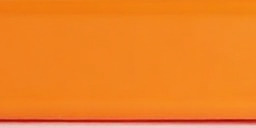
\includegraphics[width=78.500bp,height=39.250bp]{qual_tiles/nfe13/055_ours_crop.jpg}};
\node[anchor=north,inner sep=0] at (455.75,-315.80) {\num \textbf{36.15}};
\end{tikzpicture}
\end{document}
